
\def \Subject {گزارش پیاده سازی مدل }
\def \Course {درس یادگیری ماشین}
\def \Author {کسرا سینایی، امیرحسین افخمی}
\def \Report {گزارش نهایی}
\def \StudentNumber {۸۱۰۶۹۶۲۵۴، 810696206}

\begin{center}
\vspace{.4cm}
{\bf {\huge \Subject}}\\
{\bf \Large \Course}
\vspace{.2cm}
\end{center}
{\bf \Author }  \\
{\bf شماره دانشجویی:\ \StudentNumber}
\hspace{\fill} 
{\Large \Report} \\
\hrule
\vspace{0.8cm}

\clearpage

%\huge{\Subject}\\[1.5 cm]
%\chapterauthor{\Author~ : \StudentNumber}

\section{فیچر اکسترکشن}
برای رسیدن به یک مدل مناسب برای طبقه بندی و همچنین خوشه بندی، مهم ترین عامل، داشتن فیچر مناسب است.
برای استخراج فیچرهای مناسب از آهنگ‌های موجود سعی شد تا تمامی فیچرهای اصلی ممکن استخراج شود.
در مجموع 97 فیچر از آهنگ‌های موجود در دیتاست استخراج شد که در ادامه آورده شده‌اند.
لازم به ذکر است که به طور کلی دو رویکرد برای استخراج ویژگی از داده‌های صوتی وجود دارد که یکی از آن‌ها مطابق رویکردی است که در این پروژه اتخاذ شده است ودیگری 
تبدیل داده‌های صوتی به صورت فریم‌های تصویری و استفاده از این تصاویر برای تسک‌های یادگیری ماشین است.
از آن جایی که استفاده از شبکه‌های کانولوشنی در این پروژه مجاز نیست، در این جا از این روش استفاده نشد.

در فیچرهای زیر، مقادیر واریانس و میانگین به عنوان فیچر برای هر یک از آهنگ‌ها در نظر گرفته شد.

\begin{description}

    \item[$\bullet$] \lr{Chroma STFT}
    \item[$\bullet$] \lr{Spectral Centroid} 
    \item[$\bullet$] \lr{Spectral Rolloff}
    \item[$\bullet$] \lr{Spectral Bandwidth}
    \item[$\bullet$] \lr{Zero Crossing Rate}
    \item[$\bullet$] \lr{RMS Value for Each Frame}
    \item[$\bullet$] \lr{Roll-Off Frequency}
    \item[$\bullet$] \lr{Tempo}
    \item[$\bullet$] \lr{Pulse}  
    \item[$\bullet$] \lr{Harmony}
    \item[$\bullet$] \lr{:Mel-Frequency Cepstral Coefficients}
    در این فیچر میانگین و واریانس 20 \lr{MFCC} اول به عنوان فیچر در نظر گرفته شدند.
    \item[$\bullet$] \lr{:Mel-Scaled Spectrogram} 
    در این جا نیز همچون \lr{MFCC}، میانگین و واریانس 20 فیچر اول به عنوان فیچر در نظر گرفته شدند.

\end{description}

در نهایت برای هر یک از آهنگ‌ها به طور جداگانه فیچرهای فوق استخراج شدند و در یک فایل CSV ذخیره شدند.
در پایان باید به این نکته توجه داشت که تمامی فیچرهای اکسترکت شده مناسب نیستند و به اصطلاح فیچر خوبی برای تسک کلسیفیکیشن به حساب نمیایند، چرا که 
\lr{ِDiscriminability} لازم را ایجاد نمی‌کنند. برای این موضوع در قسمت‌های بعدی، تمهیداتی همچون فیچر سلکشن و فیچر ریداکشن اندیشیده شده است.

\section{پیش پردازش}




\subsection{\lr{Feature Selection}}
برای پیدا کردن بهترین فیچرهای موجود برای رسیدن به بیشترین میزان دقت طبقه بند، در این جا از تکنیک \lr{Sequential Forward Selection} استفاده شد.
برای بهینه تر کردن انتخاب فیچرها، از \lr{Floating} نیز استفاده شد.
معیار انتخاب ویژگی‌عا در فرایند فیچر سلکشن، میزان دقت طبقه بند \lr{SVM} با کرنل \lr{Linear} در نظر گرفته شد. 
به این صورت 40 فیچر اول انتخاب شدند، همچنین برای انتخاب این فیچرها از 5 \lr{Cross Validation} نیز استفاده شد.
در ادامه نمودار مربوط به دقت مدل به ازای فیچر انتخابی آورده شده است.

\begin{figure}[h!]
    \centering
    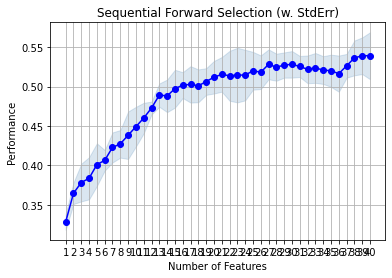
\includegraphics[width=1\linewidth]{images/feature_selection.png}
    \caption{انتخاب فیچرها با استفاده از \lr{SFS}}
    \label{fig:feature_selection}
\end{figure}



\section{طبقه بندی}

برای طبقه بندی از 3 الگوریتم مختلف استفاده شد. الگوریتم‌های مورد استفاده شامل \lr{SVM}، \lr{KNN} و \lr{MLP} بودند.
نتایج حاصل برای هر یک از 3 الگوریتم طبقه بند در ادامه آورده شده است.
\subsection{\lr{:SVM}}
الگوریتم \lr{soft-SVM} با استفاده از کرنل‌های مختلف پیاده سازی شد. بهترین دقت حاصل 
با در نظر گفتن کرنل \lr{Linear} و مقدار ترم \lr{Regularization} 5 بود که برابر با 55 درصد شد.
\lr{Confusion Matrix} مربوط به این طبقه بند در ادامه آورده شده است.

\begin{figure}[h!]
	\centering
	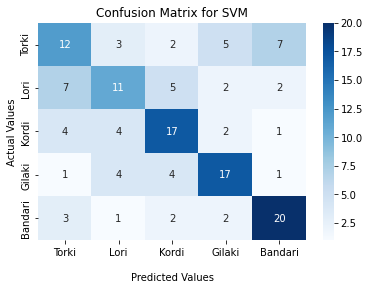
\includegraphics[width=1\linewidth]{images/svm_confusion_matrix.png}
	\caption{ماتریس کانفوژن برای الگوریتم \lr{SVM}}
	\label{fig:svm_confusion_matrix}
\end{figure}

میزان دقت، \lr{Precision}، \lr{Recall} و \lr{F1-score} برای این طبقه بند نیز در ادامه آورده شده است.

\begin{figure}[h!]
	\centering
	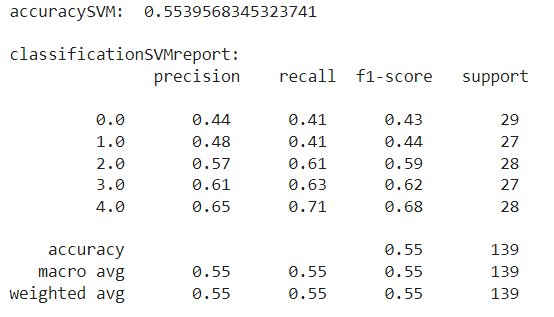
\includegraphics[width=1\linewidth]{images/svm_scores.PNG}
	\caption{میزان دقت، \lr{Precision}، \lr{Recall} و \lr{F1-score} برای الگوریتم \lr{SVM}}
	\label{fig:svm_scores}
\end{figure}

نتایج حاصل به دست آمده با استفاده از کرنل \lr{RBF} برای الگوریتم \lr{SVM} نیز در ادامه آورده شده است.

\newpage

\begin{figure}[h!]
	\centering
	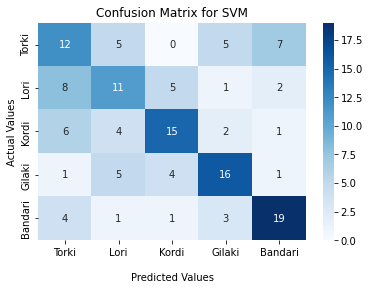
\includegraphics[width=1\linewidth]{images/svm_rbf_confusion_matrix.png}
	\caption{ماتریس کانفوژن به دست آمده با استفاده از کرنل \lr{RBF} برای الگوریتم \lr{SVM}}
	\label{fig:svm_rbf_confusion_matrix}
\end{figure}

\begin{figure}[h!]
	\centering
	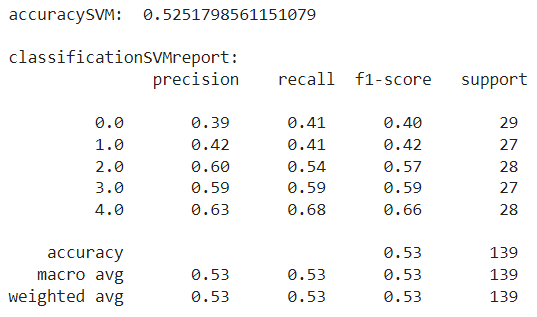
\includegraphics[width=1\linewidth]{images/svm_rbf_scores.PNG}
	\caption{نتایج حاصل به دست آمده با استفاده از کرنل \lr{RBF} برای الگوریتم \lr{SVM}}
	\label{fig:svm_rbf_scores}
\end{figure}

\newpage

\subsection{\lr{:KNN}}
در این الگوریتم، بیشترین میزان دقت با استفاده از در نظر گرفتن نزدیک ترین همسایه بیشترین میزان دقت بدست آمد که برابر با 51 درصد شد. 
متریک در نظر گرفته شده برای الگوریتم نزدیک ترین همسایه، فاصله اقلیدسی در نظر گرفته شد.
نتایج حاصل از طبقه بند نزدیک ترین همسایه در ادامه آورده شده است.

\begin{figure}[h!]
	\centering
	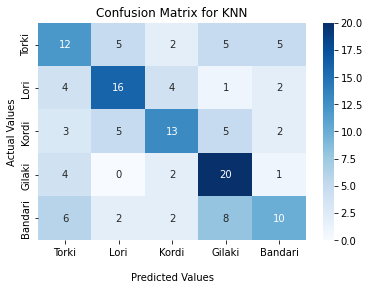
\includegraphics[width=1\linewidth]{images/knn_confusion_matrix.png}
	\caption{ماتریس کانفوژن برای الگوریتم \lr{KNN}}
	\label{fig:knn_confusion_matrix}
\end{figure}

\newpage

\begin{figure}[h!]
	\centering
	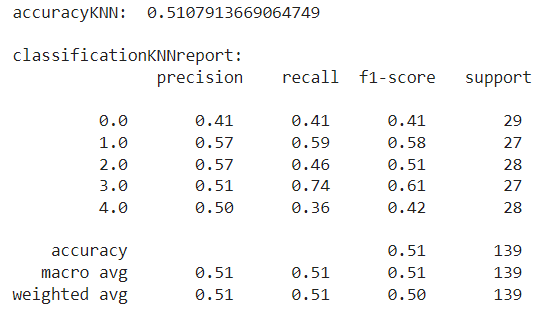
\includegraphics[width=1\linewidth]{images/knn_scores.PNG}
	\caption{نتایج حاصل به دست آمده برای الگوریتم \lr{KNN}}
	\label{fig:knn_scores}
\end{figure}

\newpage

\subsection{\lr{:MLP}}
ساختار شبکه در نظر گرفته شده برای این الگوریتم، یک ساختار سه لایه با 128، 64 و 32 نورون در لایه پنهان است. همچنین تابع فعالساز 
\lr{ReLu} برای نورون‌های شبکه طراحی شده در نظر گرفته شد.
بین تمام لایه‌های پنهان نیز لایه دراپ اوت جهت جلوگیری از اورفیت مدل قرار داده شد. مدل در 1000 ایپاک و در بچ‌های 64 تایی آموزش داده شد.
نتایج حاصل در ادامه آورده شده است.

\begin{figure}[h!]
	\centering
	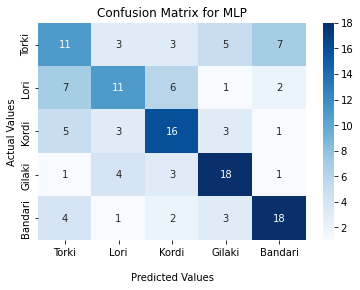
\includegraphics[width=1\linewidth]{images/mlp_confusion_matrix.png}
	\caption{ماتریس کانفوژن برای الگوریتم \lr{MLP}}
	\label{fig:mlp_confusion_matrix}
\end{figure}

\begin{figure}[h!]
	\centering
	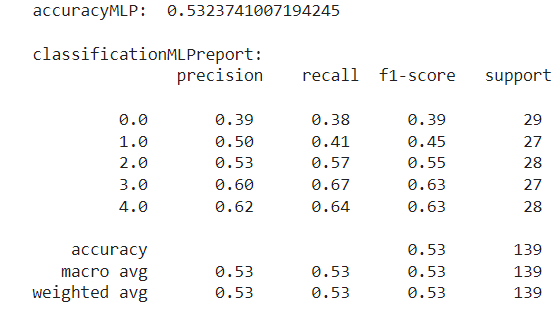
\includegraphics[width=1\linewidth]{images/mlp_scores.PNG}
	\caption{نتایج حاصل به دست آمده برای الگوریتم \lr{MLP}}
	\label{fig:mlp_scores}
\end{figure}



میتوان دید که بیشترین دقت به دست آمده نزدیک 55 درصد بود که دقت بسیار پایینی است. علت آن را می‌توان در فیچرهای کاهش یافته و به نمایش در آمده
در \lr{PCA} و \lr{LDA} دید. همان طور که مشخص است، فیچرها از \lr{ِDiscriminability} چندانی برخوردار نیستند
و کم بودن دیتا نیز عاملی افزاینده بر این مشکل است.

\section{خوشه بندی}

\section{نمایش داده ها در ابعاد پایین تر} 





\section{\lr{:Data Augmentation}}
برای حل مشکل کمبود داده، بر روی داده‌ها دیتا آگمنتیشن انجام شد، به این صورت که هر آهنگ به 5 بخش تقسیم شد و فیچرهای مورد نظر 
به صورت جداگانه از هر یک از این بخش‌ها استخراج شدند. با این کار عملا داده‌ها 5 برابر شدند. همان طور که میدانیم، برخلاف تعداد فیچر،
تعداد داده هر چقدر بیشتر باشد، کارایی مدل ما بهتر است.
این تاثیر را می‌توان در مدل‌های پیاده سازی شده در ادامه دید.

\subsection{\lr{: classification}}
نتایج حاصل از طبقه بندی با استفاده از داده‌های اضافه شده برای هر یک از الگوریتم‌ها در ادامه آورده شده است.

\subsubsection{\lr{: SVM}}
با در نظر گرفتن ترم \lr{Regularization} = 15 و 
کرنل \lr{rbf} در الگوریتم \lr{soft-SVM}
نتایج زیر حاصل گشت.



\begin{figure}[h!]
	\centering
	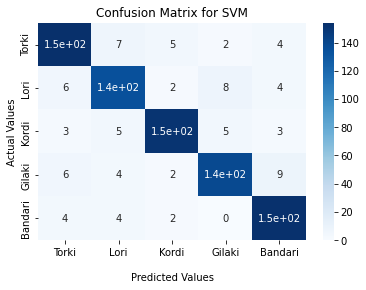
\includegraphics[width=1\linewidth]{images/svm_cm_augment.png}
	\caption{ماتریس کانفیوژن دست آمده برای الگوریتم \lr{SVM}}
	\label{fig:svm_cm_augment}
\end{figure}


\begin{figure}[h!]
	\centering
	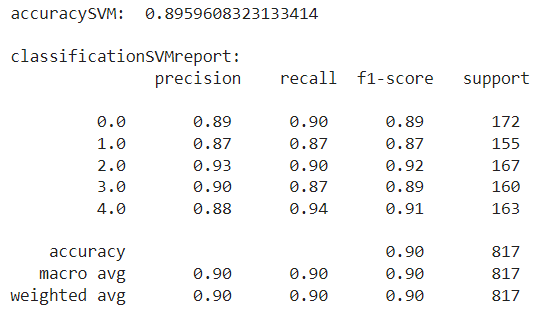
\includegraphics[width=1\linewidth]{images/svm_classification_results_augment.PNG}
	\caption{نتایج حاصل به دست آمده برای الگوریتم \lr{SVM}}
	\label{fig:svm_classification_results_augment}
\end{figure}

\subsubsection{\lr{: MLP}}
ساختار شبکه در اینجا دو لایه با 128 و 32 نورون به همراه توابع فعالساز \lr{ReLu} در نظر گرفته شد.
نتایج این طبقه بند در ادامه آورده شده است.

\begin{figure}[h!]
	\centering
	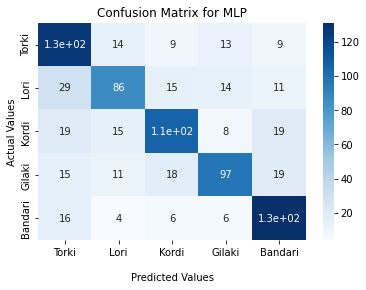
\includegraphics[width=1\linewidth]{images/mlp_cm_augment.png}
	\caption{ماتریس کانفیوژن دست آمده برای الگوریتم \lr{MLP}}
	\label{fig:mlp_cm_augment}
\end{figure}

\begin{figure}[h!]
	\centering
	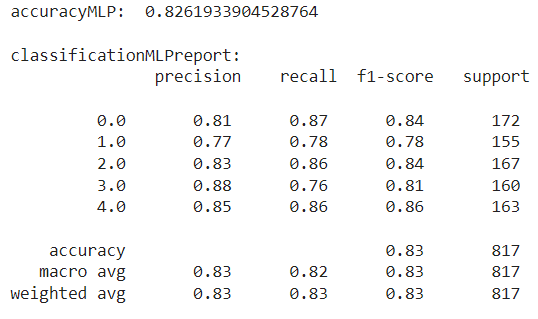
\includegraphics[width=1\linewidth]{images/mlp_classification_results_augment.PNG}
	\caption{نتایج حاصل به دست آمده برای الگوریتم \lr{MLP}}
	\label{fig:mlp_classification_results_augment}
\end{figure}

\subsubsection{\lr{: KNN}}
نتایج الگوریتم \lr{KNN} با در نظر گرفتن \lr{k=1} در ادامه آورده شده است.

\begin{figure}[h!]
	\centering
	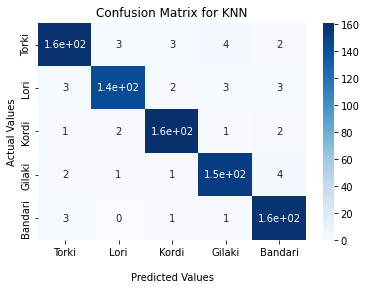
\includegraphics[width=1\linewidth]{images/knn_cm_augment.png}
	\caption{ماتریس کانفیوژن دست آمده برای الگوریتم \lr{KNN}}
	\label{fig:knn_cm_augment}
\end{figure}

\begin{figure}[h!]
	\centering
	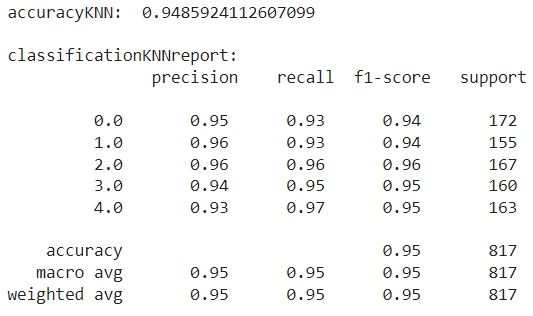
\includegraphics[width=1\linewidth]{images/knn_classification_results_augment.PNG}
	\caption{نتایج حاصل به دست آمده برای الگوریتم \lr{KNN}}
	\label{fig:knn_classification_results_augment}
\end{figure}

میتوان دید که اضافه کردن داده تاثیر بسیار چشم گیری در عملکرد مدل‌ها دارد، به نحوی که به طور مثال در 
الگوریتم \lr{KNN} توانستیم از دقت 51 درصد به دقت 95 درصد برسیم.
این رشد چشمگیر در سایر الگوریتم‌های طبقه بندی نیز قابل رویت است.
